% Chapter X

\chapter{Validation of the Heat Flux Partitioning Model} % Chapter title

\label{ch:HFP_validation} % For referencing the chapter elsewhere, use \autoref{ch:name} 

\minitoc

%----------------------------------------------------------------------------------------

In this Chapter, we want to assess the validity of the new Heat Flux Partitioning formulation proposed in Chapter \ref{chap:HFP_Assembling}. To do so, we will conduct two different validations:

\begin{itemize}
\setlength{\itemsep}{8pt}
\item The first part will be dedicated to validation on a single experimental subcooled boiling case at 10.5 bar from Kossolapov \cite{kossolapov_experimental_2021} for which numerous physical parameters have been measured. This will ensure that the mathematical formulation and the closure laws propose an acceptable physical modeling of the boiling parameters.

\item The second part will consist on wall temperature predictions for vertical subcooled flow boiling of water in various conditions, including pressure. Experimental database from Jens \& Lottes \cite{jens_analysis_1951}, Kennel \cite{kennel_local_1949} and Kossolapov \cite{kossolapov_experimental_2021}. Comparison with other HFP models from Kurul \& Podowski, Basu and Kommajosyula will be performed.
\end{itemize}


\section{Detailed Comparison and Assessment of the Heat Flux Partitioning}
\label{sec:hfp_valid_fullkoss}

In this section, we compare our results to those obtaines by Kossolapov \cite{kossolapov_experimental_2021} in vertical subcooled flow boiling. At a pressure of 10.5 bar, he realized measurements of many relevant parameters regarding the Heat Flux Partitioning:

\begin{itemize}
\item Active nucleation site density $N_{sit,a}$ ;
\item Bubble nucleation frequency $f$ ;
\item Bubble wait time $t_{w}$ ;
\item Transient heat transfer (quenching) time $t_{q}$ ;
\item Average bubble growth time $t_{g}$ ;
\item Average area visited by a bubble $A_{q,1b}$ ;
\item Proportion of the heater area impacted by bubbles $A_{b,tot}$
\item Liquid single-phase heat flux proportion $\dfrac{\phi_{c,L}}{\phi_{w}}$ ;
\item Quenching heat flux proportion $\dfrac{\phi_{q}}{\phi_{w}}$ ;
\item Wall superheat $\Delta T_{w}$.
\end{itemize}

The only lacking parameters to conduct a full evaluation of the model would be the average bubble departure diameter $R_{d}$, sliding length $l_{sl}$ and lift-off diameter / coalescence diameter.

The values provided by Kossolapov are an average conducted over all the observed nucleation events during the time of the experiment. Such data are representative of what we want to achieve using a HFP model since we represent average values of the boiling parameters for the considered boiling surface.

\npar

All those variables were measured for a subcooling $\Delta T_{L} = 10\degC$ at three different liquid mass fluxes $G_{L} = 500$, $1000$ and $2000~\debm$. 

\npar

\textbf{In next Subsections, we present the results obtained by comparison with the case at $G_{L} = 2000\ \debm$ for each of those variables. The simulations using the HFP model were conducted using a contact angle $\theta = 85 \degree$ (usual contact angle for water and ITO \cite{kossolapov_experimental_2021}), an hysteresis $\dtheta = 2 \degree$ and a growth constant $K=0.8$}

 
\subsection{Active Nucleation Site Density}

On Figure \ref{fig:fullkoss_nsit}, we compare the values obtained for the active nucleation site density. The Li \etal correlation used in the model (Eq. \ref{eq:nsit_li}) propose a reasonable prediction of the measured values of $N_{sit,a}$ with an underestimation of less than a decade. The correlation correctly reproduce the experimental trend where we observe a sort of saturation in the nucleation site density for higher wall superheat.

\npar

To better match the asymptotic value of the experiment, we correct the Li \etal correlation for this case by a factor $\Delta T_{w}^{2-0.3\Delta T_{w}^{0.5}}$ which better fits the measurements for $\Delta T_{w}>10$~K but yields a small overestimation before.


\begin{figure}[!h]
\subfloat[$N_{sit,a}$ predictions by Li \etal correlation]{
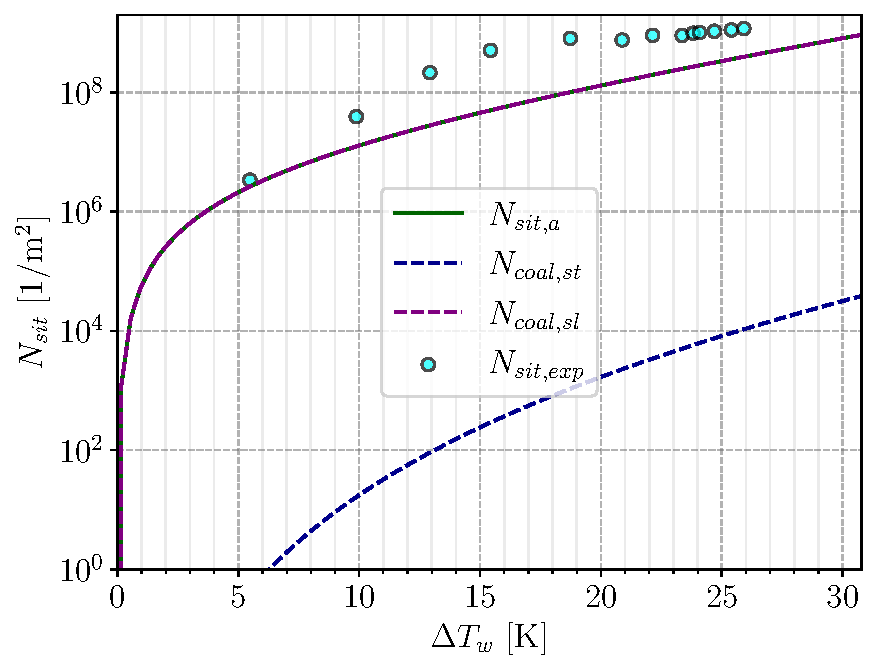
\includegraphics[width=0.5\linewidth]{img/HFP/fullcomp_Koss/sites_G2000_nocorr.pdf}
}
\subfloat[$N_{sit,a}$ predictions with corrected Li \etal correlation]{
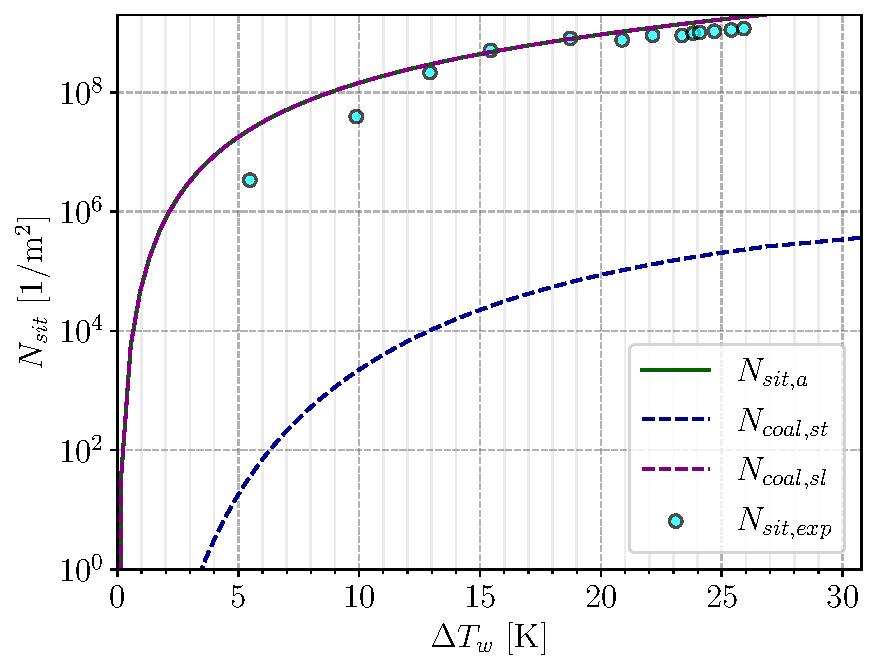
\includegraphics[width=0.5\linewidth]{img/HFP/fullcomp_Koss/sites_G2000.pdf}
}
\caption{Comparison of active nucleation site density with and without a correction for Li \etal formulation.}
\label{fig:fullkoss_nsit}
\end{figure}



\begin{note*}{}
Following comparisons are conducted using the corrected value of $N_{sit,a}$ to limit the impact of the nucleation site density prediction over the other parameters.
\end{note*}

\subsection{Wait Time, Growth Time, Quenching Time and Nucleation Frequency}

Figure \ref{fig:fullkoss_times} compares the different times involved in the boiling physics and the bubble nucleation frequency. As seen in Section \ref{sec:wait_time}, the wait time is quite fairly reproduced along with the nucleation frequency. Actually, the bubble departure is nearly instantaneous and the nucleation cycle is mainly composed of the wait period, which means a good estimation of $t_{w}$ leads to a reasonable estimation of $f$ for this case.

\npar

The average bubble growth time is overestimated by nearly a decade for low superheat and is better predicted for larger superheat. Its evolution seem coherent with a decrease up to 15\ K and a stabilization afterwards. However, the experimental measurements show an increase in the growth time for large superheat which could be associated to bubble diameter increase with the wall Jakob number as previously observed in Section \ref{sec:liftoff}. This could be in partial contradiction with the single coalescence hypothesis for the lift-off since the average distance between bubbles in likely to decrease with wall superheat, thus decreasing the average growth time. On the other hand, the growth time overprediction may be associated to sliding length overestimation, especially at low wall superheat.

\npar

A very good approximation of the quenching time $t_{q}$ is achieved using the time $t^{*}$ (Eq. \ref{eq:tstar}). This indicates that for this experimental case, the large value of the wait time implies that the transient conduction will be limited to a duration $t^{*}$ and that the remaining wait time will be governed by forced convection. 

\begin{figure}[!h]
\subfloat[Bubble nucleation frequency]{
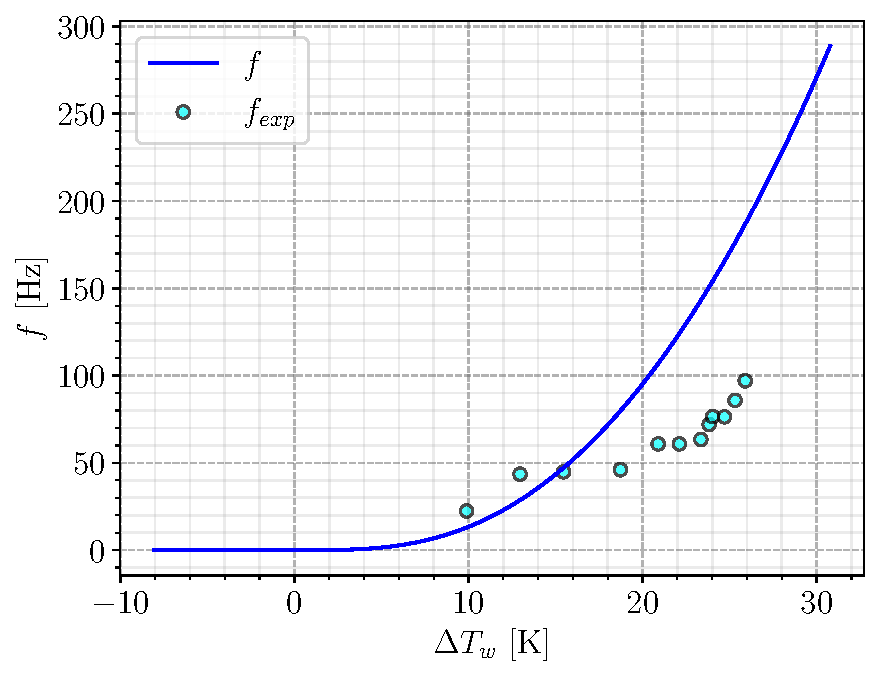
\includegraphics[height=0.35\linewidth]{img/HFP/fullcomp_Koss/f_G2000.pdf}
}
\subfloat[Bubble wait time, growth time and quenching time]{
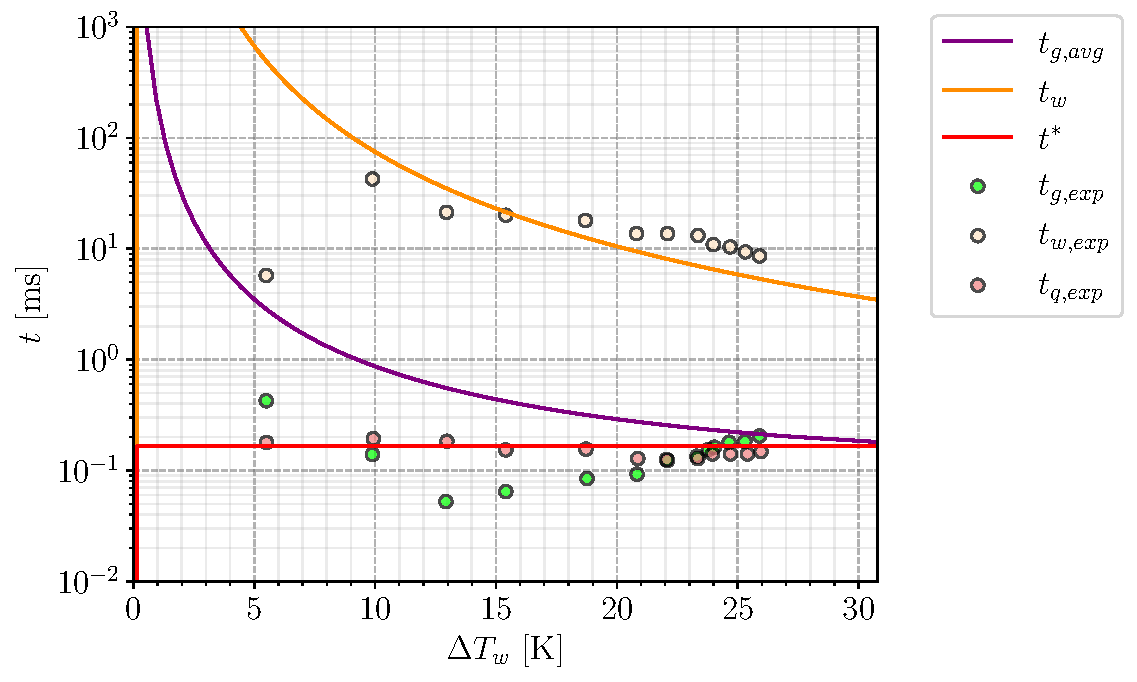
\includegraphics[height=0.35\linewidth]{img/HFP/fullcomp_Koss/times_G2000.pdf}
}
\caption{Comparison of bubble nucleation frequency, wait time, average growth time and quenching time.}
\label{fig:fullkoss_times}
\end{figure}





\subsection{Single Bubble Area and Total Bubble Area}

Figure \ref{fig:fullkoss_area} shows that the total area visited by a bubble  $A_{q,1b}$ is largely overestimated for the whole boiling curve. It only achieves a reasonable order of magnitude at high wall superheat ($\Delta T_{w} > 23\ $K). This could question the usual hypothesis that supposes a sliding length $l_{sl}$ equal to the average distance between bubbles $s_{b} = 0.5/\sqrt{N_{b}}$. The sole projected area of the bubbles is in average better for the visited area, but underpredicts the largest values of $A_{q,1b}$ when bubbles start sliding over significant lengths.

\npar

Moreover, both values do not reproduce the experimental trend where the visited area regularly increases with the wall superheat. Further experimental insights regarding the behavior of the bubble sliding length could allow a better modeling of $l_{sl}$ depending on the bubble lift-off process as discussed in Section \ref{sec:liftoff}.

\npar

Those results naturally lead to an overprediction of the wall area fraction impacted by bubbles but shows an coherent increasing trend with wall superheat.

\npar 



\begin{figure}[!h]
\subfloat[Single bubble area]{
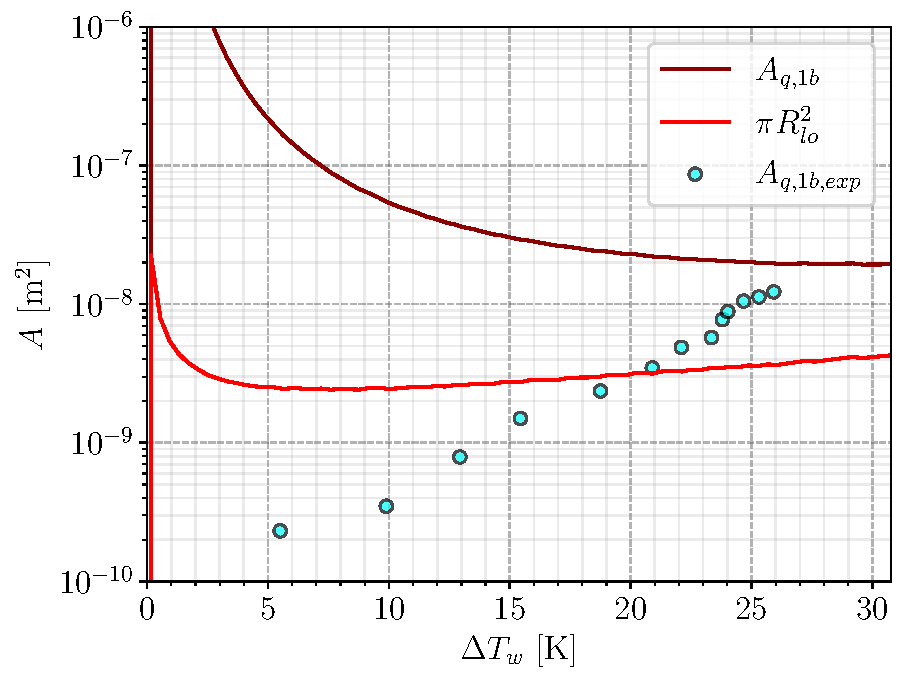
\includegraphics[width=0.5\linewidth]{img/HFP/fullcomp_Koss/Aq1b_G2000.pdf}
}
\subfloat[Total wall area impacted by bubbles]{
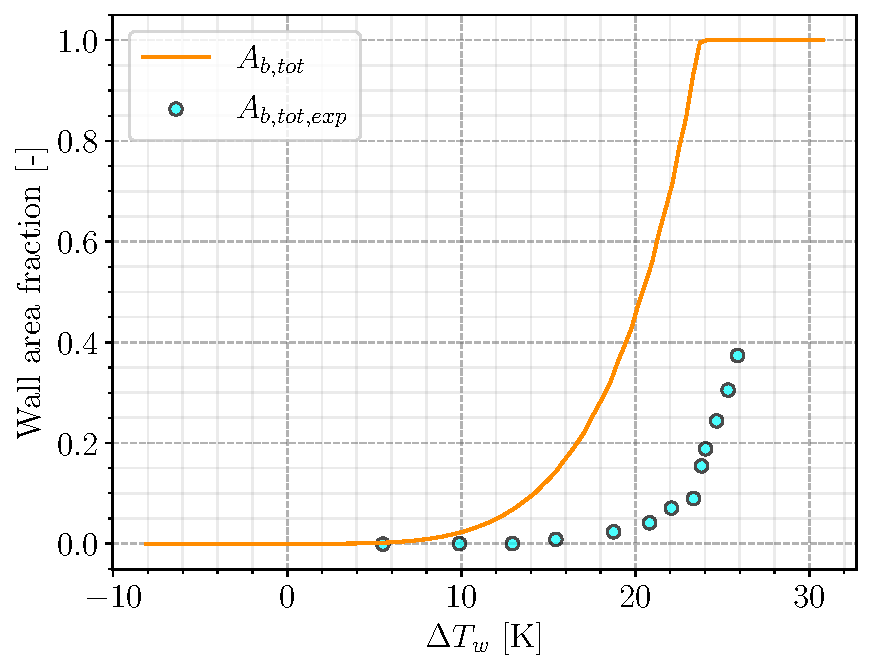
\includegraphics[width=0.5\linewidth]{img/HFP/fullcomp_Koss/Abub_tot_G2000.pdf}
}
\caption{Comparison of average area visited by a bubble and total wall fraction area impacted by bubbles (footprint or transient conduction).}
\label{fig:fullkoss_area}
\end{figure}

\npar

On Figure \ref{fig:fullkoss_length}, we indicatively show the values of sliding length $l_{sl}$, departure diameter $R_{d}$ and sliding diameter $R_{sl}$ when sliding over $l_{sl}$. The small values of $R_{d}$ are coherent with nearly immediate departure by sliding, with sliding radiuses close to $0.1$ mm.


\begin{figure}[!h]
\centering
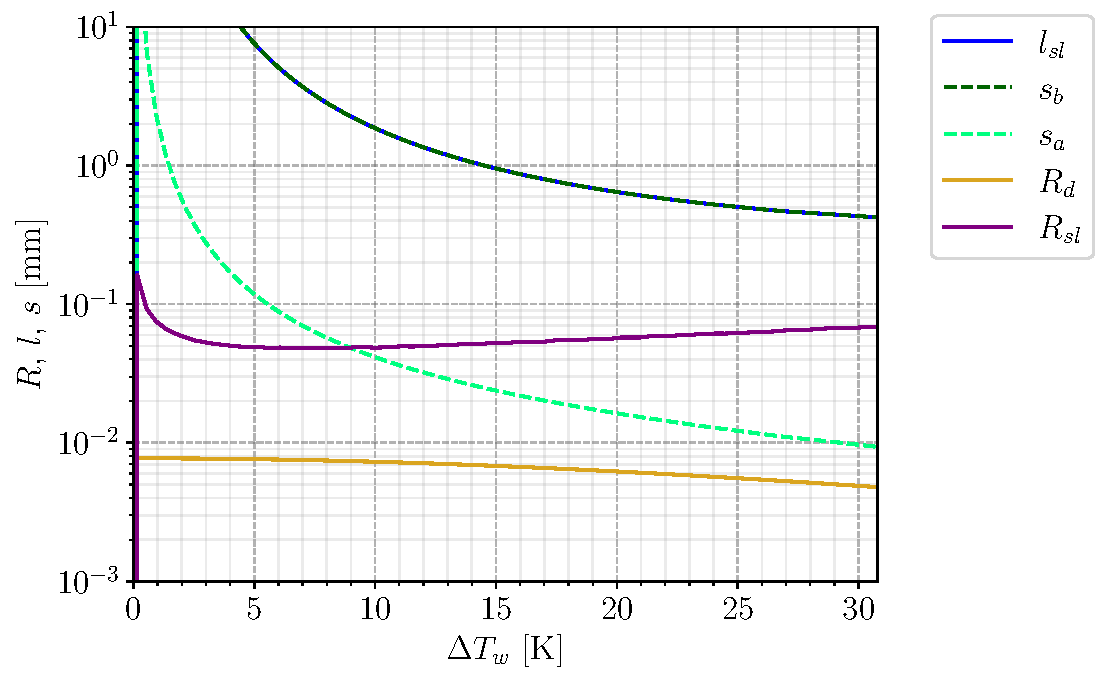
\includegraphics[width=0.65\linewidth]{img/HFP/fullcomp_Koss/length_G2000.pdf}
\caption{Bubble radiuses, sliding length and distances between sites.}
\label{fig:fullkoss_length}
\end{figure}



\subsection{Flux Proportions and Wall Superheat}

Figure \ref{fig:fullkoss_hfp} finally compares the fraction of single-phase convection and quenching over the total heat flux $\phi_{w}$ along with the boiling curve. The evolution of the single-phase flux reasonably agrees with the experiment and becomes 0 at a superheat similar to the measurement. However, the quenching heat flux is logically overestimated due to the significant overestimation of the area visited by a single bubble.

\npar

On the other hand, the boiling curve is pretty well predicted except for the last experimental measurement where an increase in wall temperature starts, which could correspond to conditions close to the CHF that can't yet be detected by the HFP model.

\begin{figure}[!h]
\subfloat[Single-phase and quenching heat fluxes proportions]{
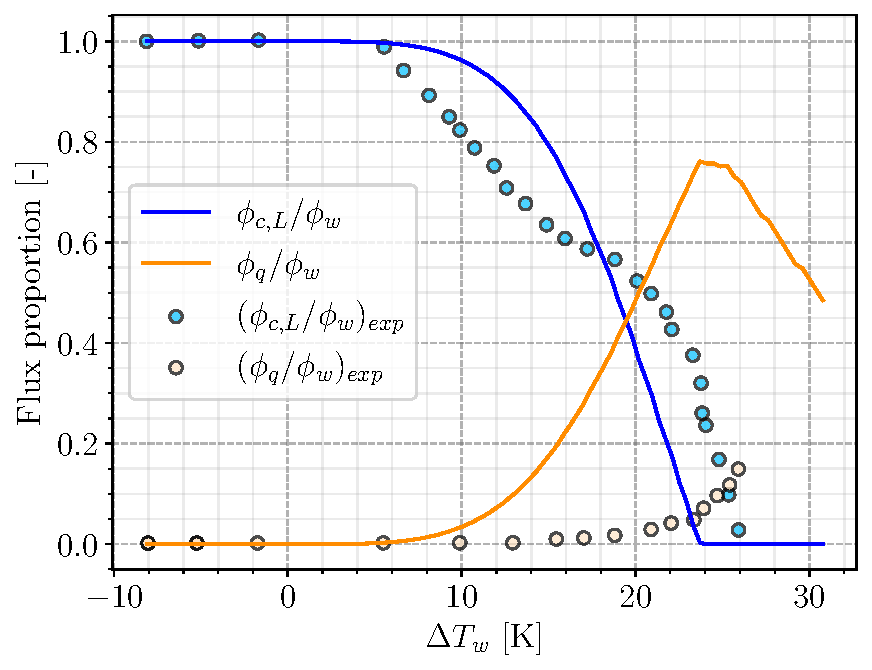
\includegraphics[width=0.5\linewidth]{img/HFP/fullcomp_Koss/hfp_G2000.pdf}
}
\subfloat[Global boiling curve of the experiment]{
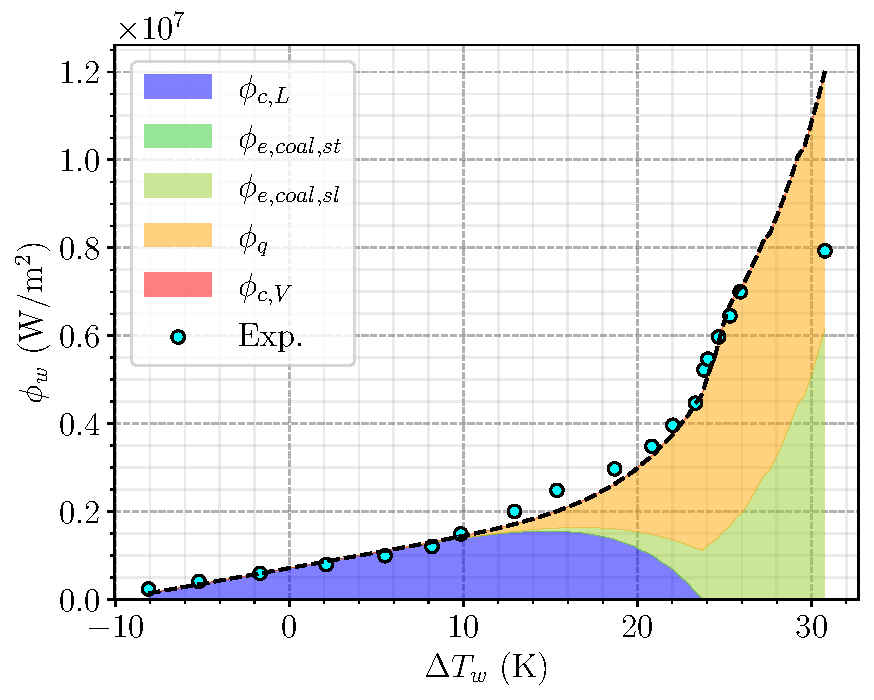
\includegraphics[width=0.5\linewidth]{img/HFP/fullcomp_Koss/boil_curve_G2000.pdf}
}
\caption{Comparison of the resulting heat flux partitioning along with the boiling curve.}
\label{fig:fullkoss_hfp}
\end{figure}


\npar

\clearpage

\section{Wall Temperature Predictions}
\label{sec:hfp_valid_DTw}

In this section, we want to evaluate the model's capability to predict wall temperature in boiling regimes for different flow conditions. To do so, we gather boiling curves data from the literature for water that covers a large range of flow conditions as detailed in Table \ref{tab:exp_data_HFP}.


\begin{table}[h!]

%\begin{changemargin}{-1cm}{0cm}

\noindent\makebox[\textwidth]{

\scriptsize
\centering
\begin{tabular}{p{20mm}|c c c c c c c c} 
Author & $D_{h}$ [mm] & $P$ [bar] & $G_{L}$ [$\debm$] & $\Delta T_{L}$ [K] & $\phi_{w}$ [MW/m\up{2}] & $\Delta T_{w}$ [K] &$N_{mes}$ [-] \\
\hline
\\

Kossolapov \cite{kossolapov_experimental_2021} \newline (2021) & 11.78 & 1.12 - 75.8 & 500 - 2000 & 10 & 0.23 - 7.93  & 1.55 - 30.77 & 81 \\

Jens-Lottes \cite{jens_analysis_1951} \newline (1951) & 5.74 & 137.9 & 2617.5 & 53.3 - 92.2 & 2.15 - 3.63 & 1.81 - 4.16 & 38 \\

Kennel \cite{kennel_local_1949} \newline (1948) & 4.3 - 13.2 & 2 - 6.2 & 284 - 10~577 & 11.1 - 83.3 & 0.053 - 6.35 & 1.64 - 49.7 & 172 \\
\hline
\end{tabular}
}
\caption{Experimental data range of wall temperature measurements in the boiling region.}
\label{tab:exp_data_HFP}
\end{table}

\npar


The following sub-sections compare the results for wall superheat predictions obtained using four models: Kurul \& Podowski (Section \ref{sec:hfp_kurul}), Basu \etal (Section \ref{sec:hfp_basu}), Kommajosyula (Section \ref{sec:hfp_komma}) and the new formulation (Section \ref{sec:hfp_new}).

\npar

In order to propose consistent choices required closing parameters for the new formulation, we will discuss the values attributed to the contact angle $\theta$, bubble inclination $\dtheta$ and constant value in bubble growth rate $K$.


\subsection{Kossolapov Data}
\label{subsec:HFP_verif_koss}

The boiling curves from Kossolapov's work \cite{kossolapov_experimental_2021} are among the most recent available data and notably include various operating pressures. The experimental setup consists of a heated flat plate of ITO in vertical flow boiling in a rectangular channel.


\npar

As stated by Kossolapov, the contact angle for water and ITO usually lies between 80$\degree$ and $90\degree$ \cite{kossolapov_experimental_2021}. The bubble tilt is likely to be very low for high pressure cases (see Sec. \ref{sec:departure}) and the bubble growth rate coefficient $K$ shall be closer to 1.5 / 2 at high pressure while it can be lower than 1 for low pressure cases. The chosen values are then:

\begin{itemize}
\item $\theta = 85 \degree$ ;
\item $\dtheta = 1 \degree$ for $P > 5\ $bar and $\dtheta = 5 \degree$ otherwise ;
\item $K = 1.5$ for $P > 5\ $bar and $K=1.0$ otherwise.
\end{itemize}


Figure \ref{fig:HFP_koss_BC} shows two typical boiling curves along with the heat flux partitioning obtained using the new formulation for Kossolapov cases at 19.8 bar and 75.8 bar.


\begin{figure}[!h]
\centering
\subfloat[$P=19.8$ bar]{
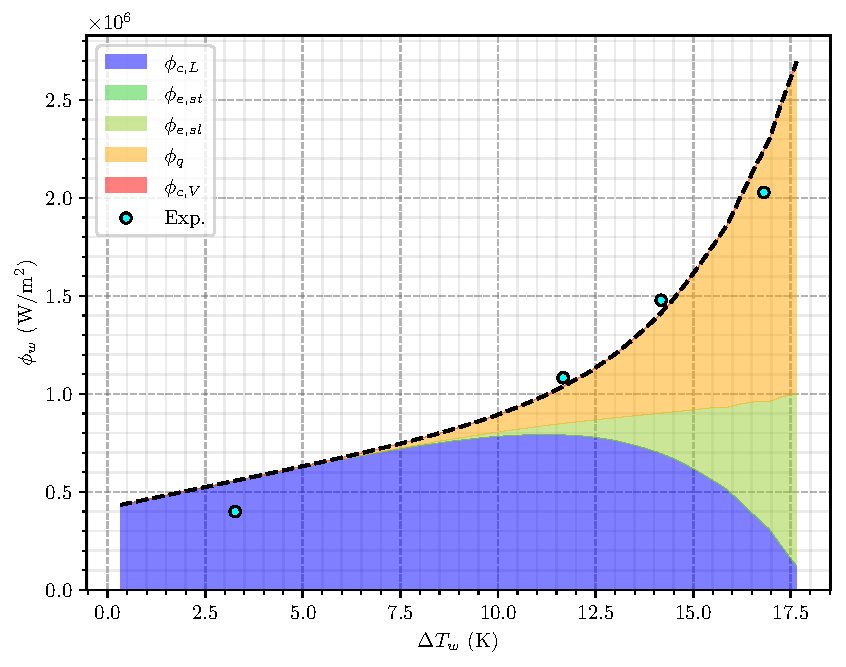
\includegraphics[width=0.5\linewidth]{img/HFP/koss/koss_p19.pdf}
}
\subfloat[$P=75.8$ bar]{
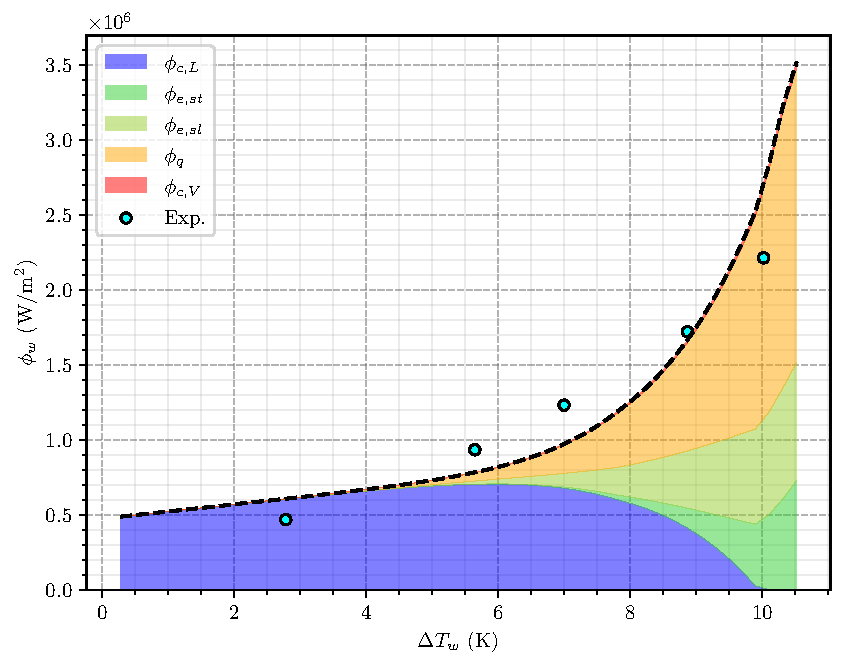
\includegraphics[width=0.5\linewidth]{img/HFP/koss/koss_p75.pdf}
}
\caption{Comparison with measured boiling curves from Kossolapov \cite{kossolapov_experimental_2021}. $\Delta T_{L}=10\degC$ and $G_{L}=1000~\debm$.}
\label{fig:HFP_koss_BC}
\end{figure}


\npar

We can observe that experimental profiles are quite fairly reproduced in both cases. The model also shows different types of heat flux partitioning with the case at 75.8 bar starting to have a significant proportion of static coalescence evaporation flux. This is probably a consequence of both the high pressure and large wall superheat resulting in a very large nucleation site density and increasing the probability for two bubbles to coalesce early in their lifetime.

\npar

Figure \ref{fig:HFP_koss} shows the wall temperature predictions achieved with the different HFP models.


\begin{figure}[!h]
\centering
\subfloat[Kurul \& Podowski]{
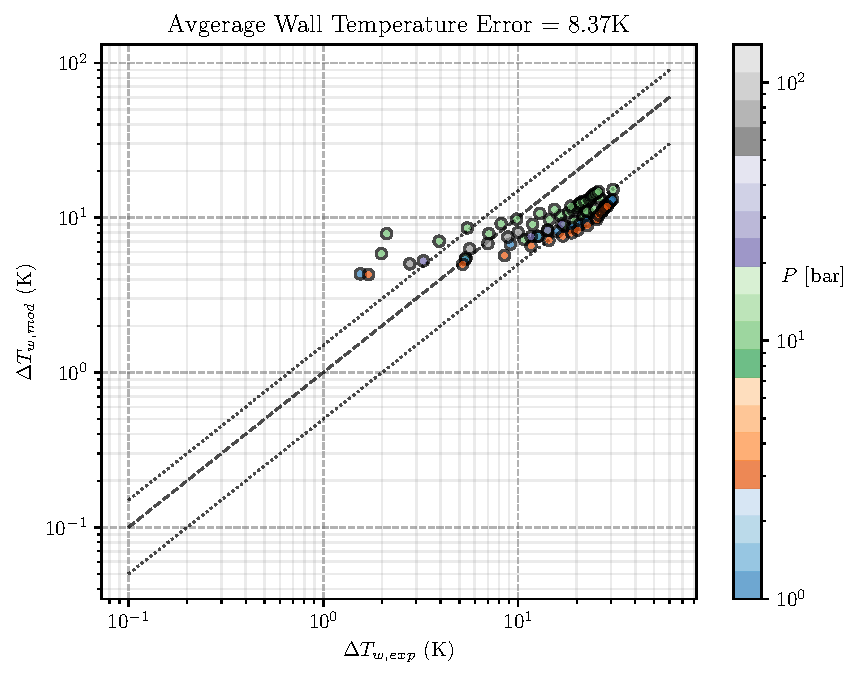
\includegraphics[width=0.5\linewidth]{img/HFP/koss/KP_Kossolapov.pdf}
}
\subfloat[Basu]{
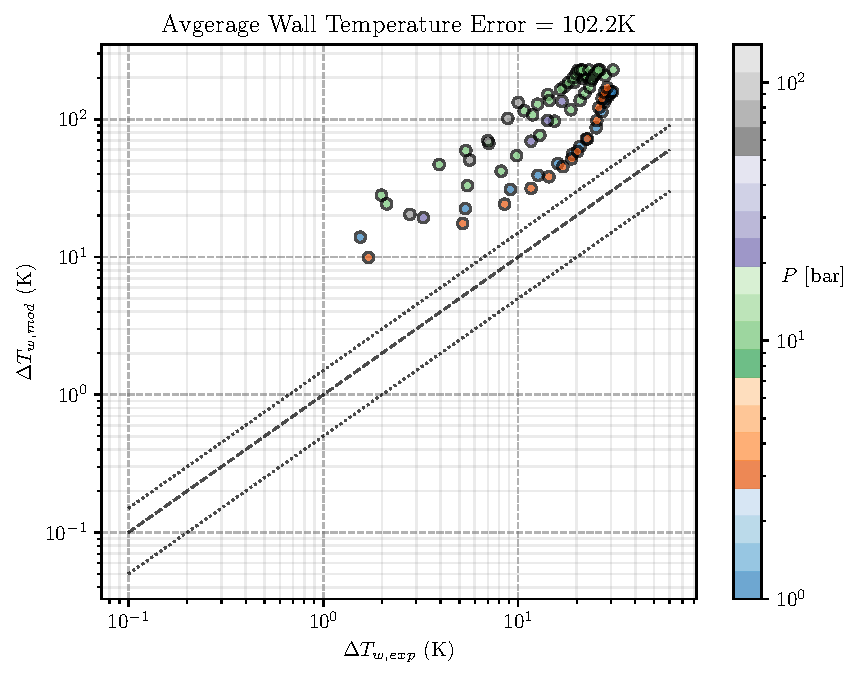
\includegraphics[width=0.5\linewidth]{img/HFP/koss/Basu_Kossolapov.pdf}
}
\\
\subfloat[Kommajosyula]{
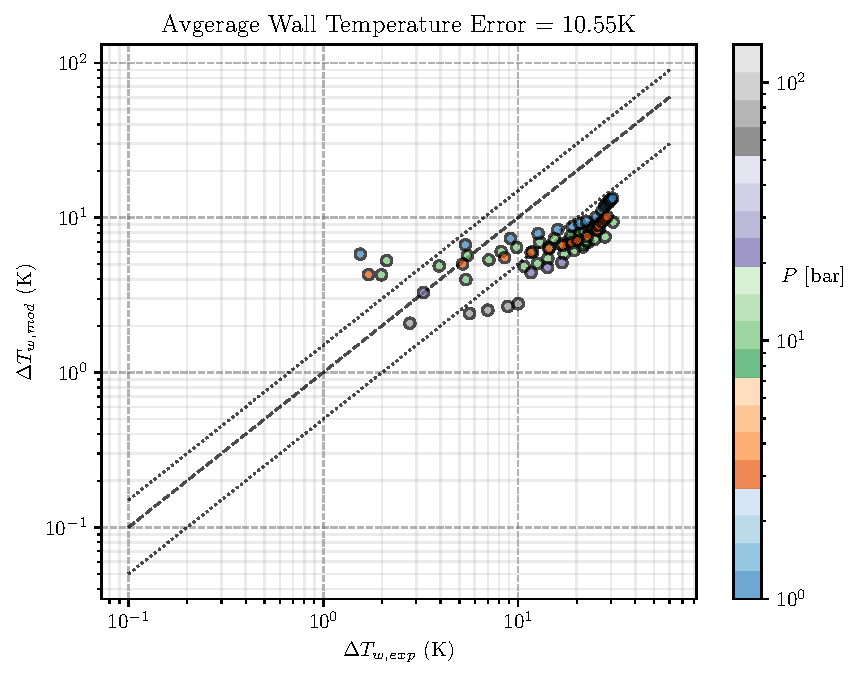
\includegraphics[width=0.5\linewidth]{img/HFP/koss/Komma_Kossolapov.pdf}
}
\subfloat[New Model]{
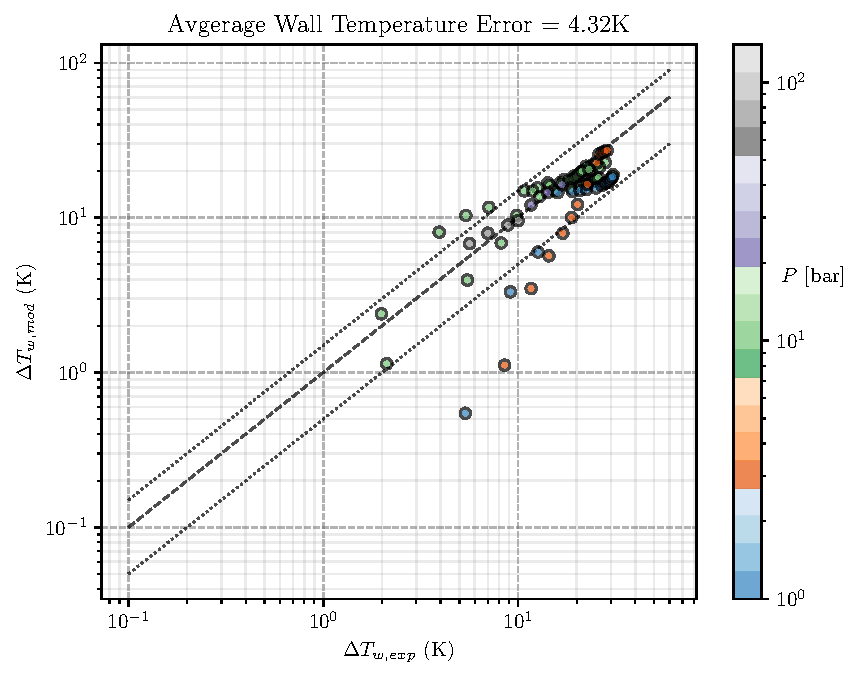
\includegraphics[width=0.5\linewidth]{img/HFP/koss/NM_Kossolapov.pdf}
}

\caption{Wall temperature predictions achieved by the different HFP models on Kossolapov data. $\pm 50\%$ error bars in dashed lines.}
\label{fig:HFP_koss}
\end{figure}

\npar
We can note that the new formulation generally better agrees with experimental measurements but yields significant underestimation of low wall superheat values for low pressure cases. The predictions achieved by Kurul \& Podowski and Kommajosyula models seem similar while Basu \etal formulation largely overestimates the wall temperature with an average error above 100~K. 




\subsection{Jens-Lottes Data}
\label{subsec:HFP_verif_Jens}

The data of Jens \& Lottes are of particular interest for the HFP validation since they were obtained in conditions close to PWR ones, with an operating pressure of 138 bar, liquid mass flux above $2500\ \debm$ and high inlet liquid subcooling. The experiment consisted of an integrally heated metallic circular pipe. Precise evaluation of the contact angle in those conditions is tricky but, according to the work of Song \& Fan \cite{song_temperature_2021}, the water contact angle on metallic surfaces (\eg stainless steel) at large pressure present a very large decrease when reaching surface temperatures above 200$\degC$. Since saturation temperature of water at 138 bar if $T_{sat} \approx 335 \degC$, the boiling measurements lie largely in the low contact angle zone. Therefore, we will assume:

\begin{itemize}
\item $\theta = 20 \degree$ ;
\item $\dtheta = 1 \degree$ (very high pressure leading to nearly non-tilted bubbles) ;
\item $K = 2.0$ (very high pressure and low Jakob numbers).
\end{itemize}


Figure \ref{fig:HFP_jens_BC} shows a typical boiling curve obtained for an experimental case of Jens \& Lottes. We can observe that in this region where wall superheat are low ($\Delta T_{w}<5\ $K), the quasi-entirety of the wall heat flux is evacuated through liquid convection and transient conduction through quenching. This is likely to be a consequence of the very high pressure conditions under which nucleation site density is very large but bubbles become extremely small ($R \sim \mu$m). Evaporation heat flux is then relatively small but the large number of bubbles and their sliding induce a strong quenching effect over the heater surface. 

\npar

\begin{figure}[!h]
\centering
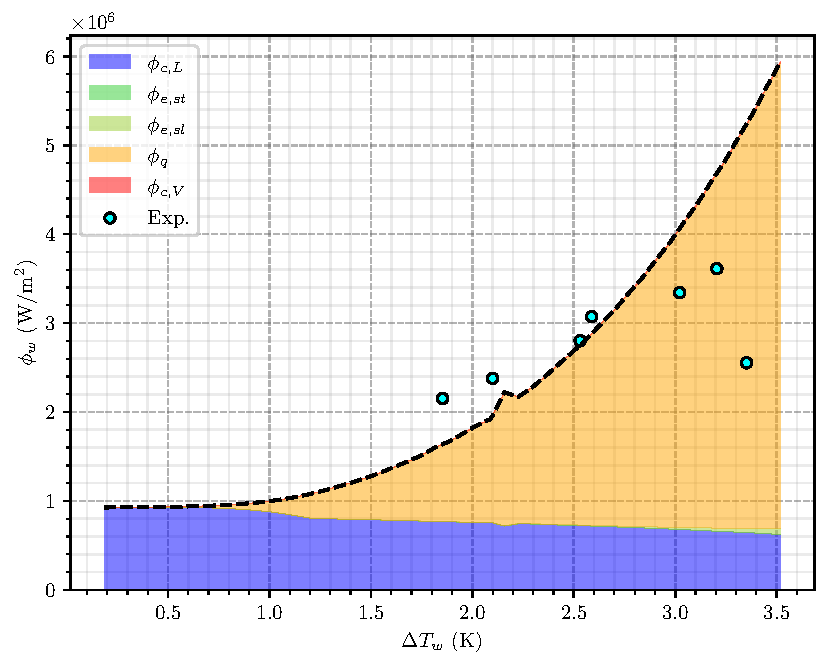
\includegraphics[width=0.6\linewidth]{img/HFP/jens/jens_p138.pdf}
\caption{Comparison with measured boiling curve by Jens \& Lottes \cite{jens_analysis_1951}. $P=138$ bar, $G=2600~\debm$, $\Delta T_{L}=64\degC$.}
\label{fig:HFP_jens_BC}
\end{figure}
\npar

Figure \ref{fig:HFP_jens} shows the wall temperature predictions achieved with the different HFP models.

\begin{figure}[!h]
\centering
\subfloat[Kurul \& Podowski]{
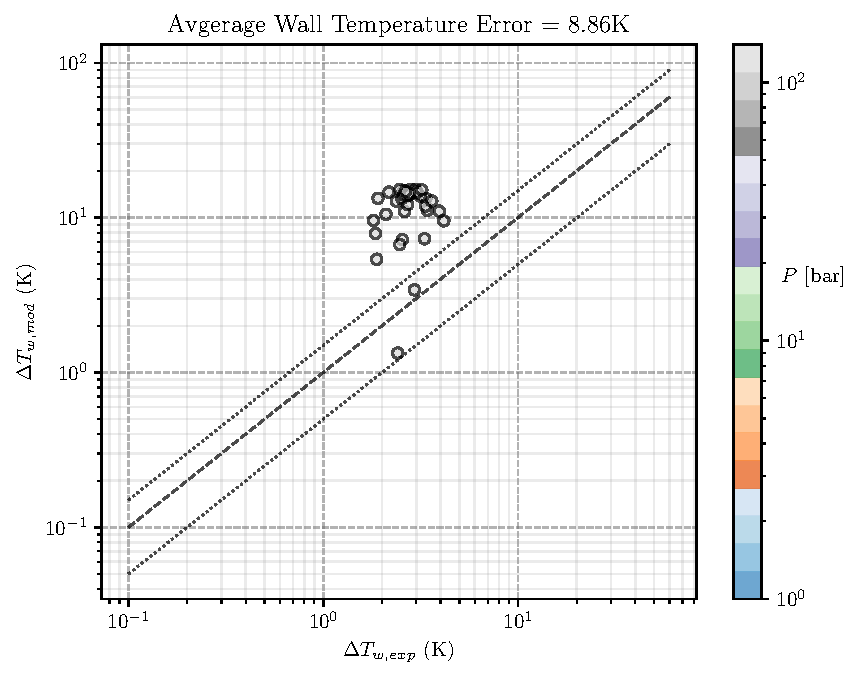
\includegraphics[width=0.5\linewidth]{img/HFP/jens/KP_Jens.pdf}
}
\subfloat[Basu]{
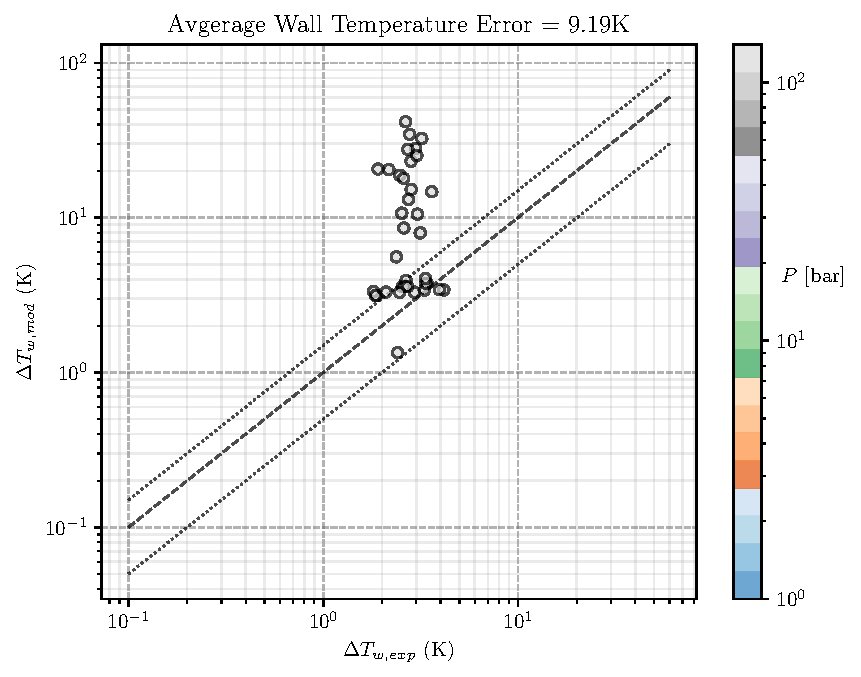
\includegraphics[width=0.5\linewidth]{img/HFP/jens/Basu_Jens.pdf}
}
\\
\subfloat[Kommajosyula]{
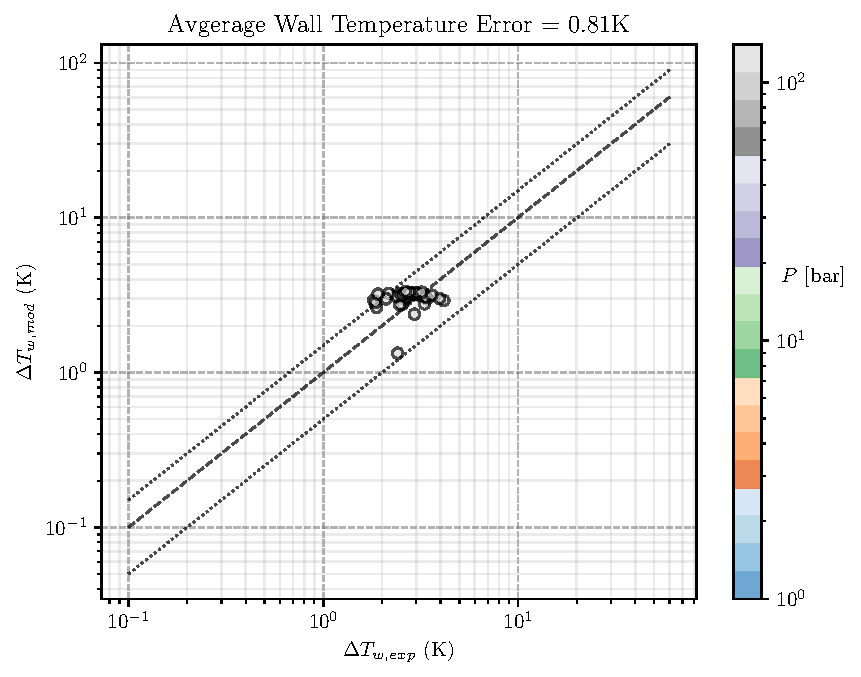
\includegraphics[width=0.5\linewidth]{img/HFP/jens/Komma_Jens.pdf}
}
\subfloat[New Model]{
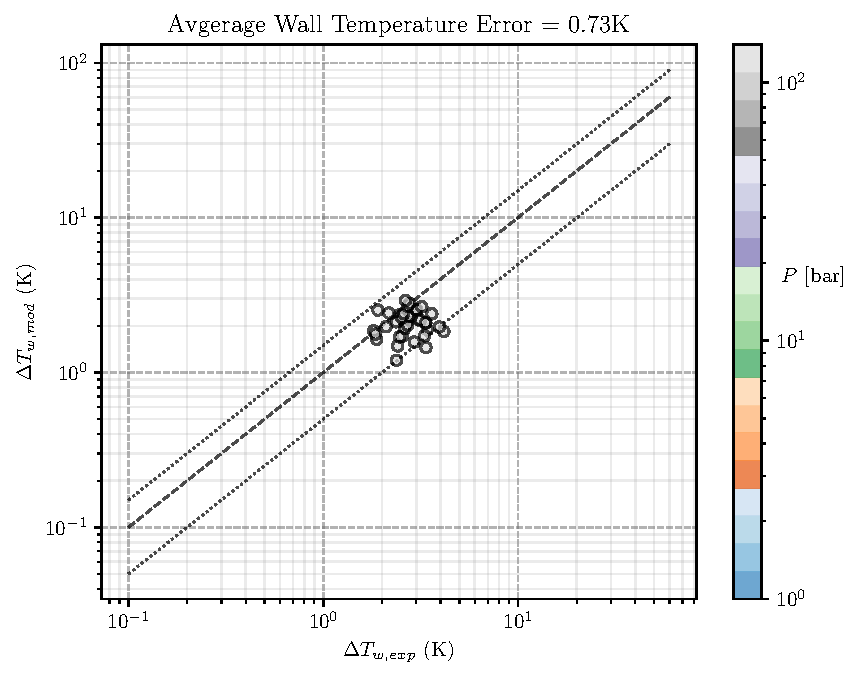
\includegraphics[width=0.5\linewidth]{img/HFP/jens/NM_Jens.pdf}
}

\caption{Wall temperature predictions achieved by the different HFP models on Jens data. $\pm 50\%$ error bars in dashed lines.}
\label{fig:HFP_jens}
\end{figure}

\npar

Both the new formulation and Kommajosyula model achieve good predictions of the wall temperature in those high pressure conditions. However, Kurul \& Podowski and Basu models do not seem to capture properly the wall superheat evolution, with large relative overestimations ($\sim 200\%$).


\subsection{Kennel Data}
\label{subsec:HFP_verif_kennel}

Kennel measurements are of similar nature to those of Jens \& Lottes since they were conducted for a uniformly heated vertical circular metallic pipe. However, the experiments were operated at pressures lower than 6 bar and various inlet liquid mass fluxes and subcoolings. In those conditions, the evaluation of the constant $K$ in the bubble growth profile can be very tricky since the larger bubbles at low pressure are more impacted by the bulk flow, implying potentially large variations of $K$ that can become much lower than 1. Regarding the contact angle, its value can also be roughly estimated using Song \& Fan review \cite{song_temperature_2021} showing that metallic surfaces at low and moderate pressure also show a contact angle decrease with temperature, with values roughly lying between $40 \degree$ and $60 \degree$ when $T_{w} \sim T_{sat}$. Therefore, we assume:


\begin{itemize}
\item $\theta = 50 \degree$ ;
\item $\dtheta = 5 \degree$ (larger and deformable bubbles at low pressure) ;
\item $K = 0.3$ (larger impact of bulk subcooling on bubble growth).
\end{itemize}



\npar



Figure \ref{fig:HFP_kennel} shows the wall temperature predictions achieved with the different HFP models.

\begin{figure}[!h]
\centering
\subfloat[Kurul \& Podowski]{
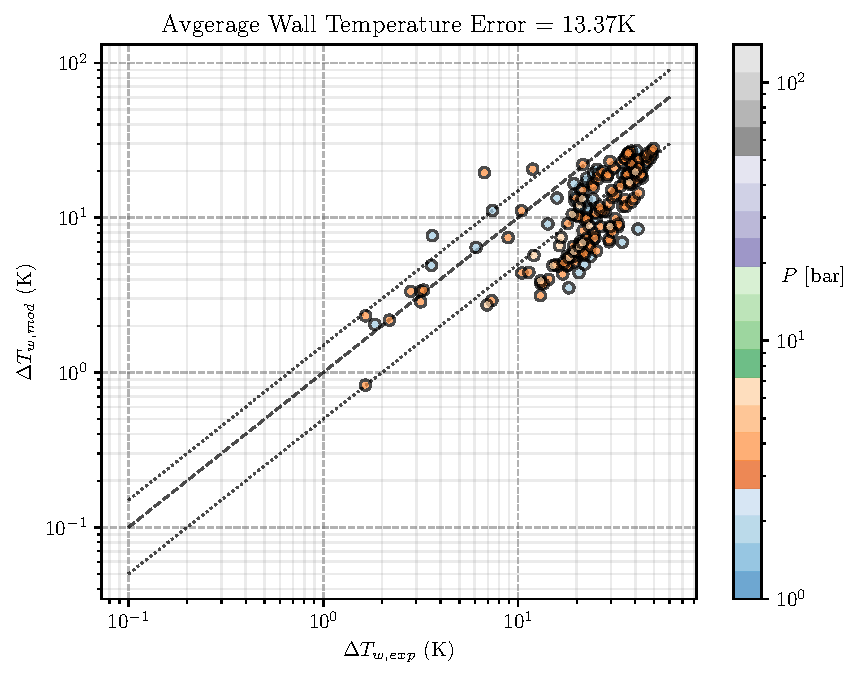
\includegraphics[width=0.5\linewidth]{img/HFP/kennel/KP_Kennel.pdf}
}
\subfloat[Basu]{
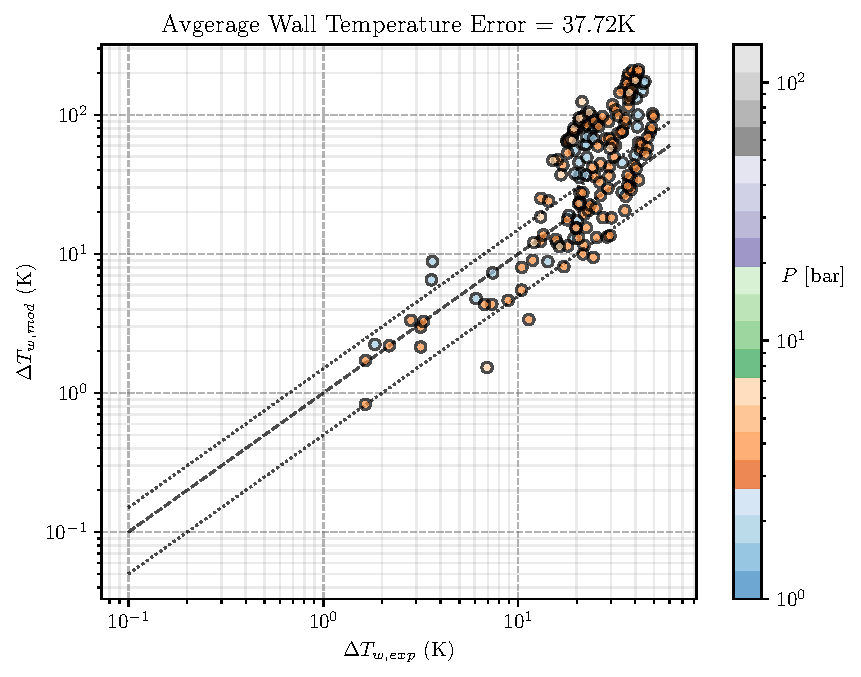
\includegraphics[width=0.5\linewidth]{img/HFP/kennel/Basu_Kennel.pdf}
}
\\
\subfloat[Kommajosyula]{
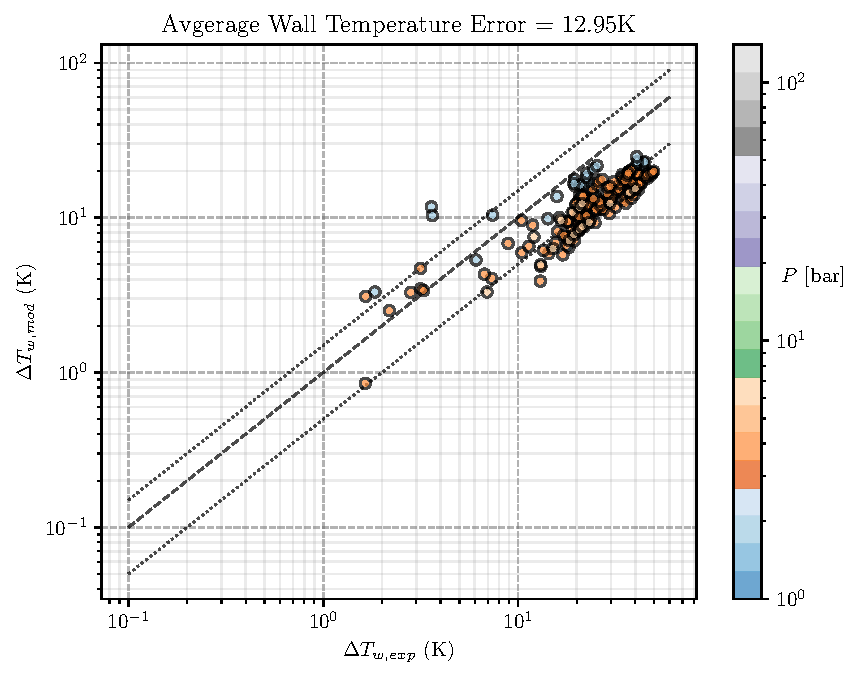
\includegraphics[width=0.5\linewidth]{img/HFP/kennel/Komma_Kennel.pdf}
}
\subfloat[New Model]{
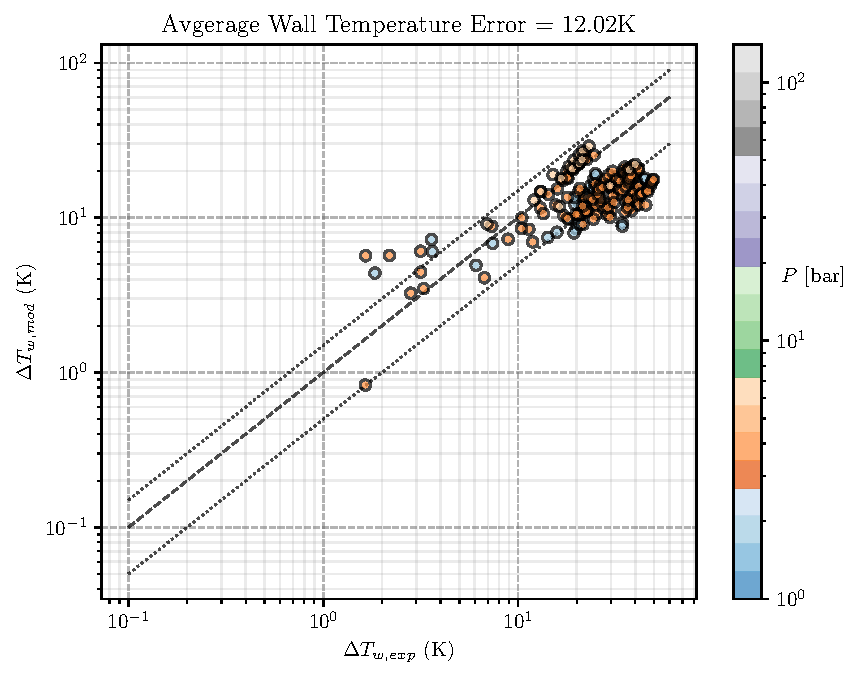
\includegraphics[width=0.5\linewidth]{img/HFP/kennel/NM_Kennel_t50_K05_dt5.pdf}
}

\caption{Wall temperature predictions achieved by the different HFP models on Kennel data. $\pm 50\%$ error bars in dashed lines.}
\label{fig:HFP_kennel}
\end{figure}

\npar

Achieving a good quality of wall superheat predictions for the cases of Kennel appears more complicated. Indeed, the new formulation and Kommajoysula model obtain the best results but still present an average underestimation of approximately 50\%. The very large range of conditions associated to the low pressure may invalidate the assumption of constants values for $\dtheta$ and $K$. 


\begin{remark*}{}
In his work, Kommajosyula \cite{kommajosyula_development_2020} presented better wall temperature predictions on Kennel data with his model (average error between 3\ K and 5\ K). We only managed to achieve similar results using a much lower contact angle ($\theta \leq 20\degree$) which could be questioned regarding the operating conditions.
\end{remark*}


\clearpage
\section{Validation for DEBORA Experiment}
\label{sec:hfp_valid_debora}

In order to try a further validation of the proposed HFP model, we will test it under conditions that are representative of the DEBORA cases for the G2P26W16 campaign (Chapter \ref{chap:debora}):


\begin{itemize}
\item R12 as operating fluid ;
\item $P=26.2\ $bar ;
\item $G_{L} = 2000~\debm$ ;
\item $\phi_{w} = 73.9\ $kW/m\up{2}.
\end{itemize}


Since refrigerant are usually known to have low contact angle and recalling that wall temperature in this case is less than $20\degC$ lower than R12 critical temperature ($T_{crit,R12} \approx 380\ $K), we suppose $\theta = 5 \degree$. The operating pressure being experimentally chosen to match high-pressure water similarity, we thus choose $\dtheta = 1 \degree$ and $K = 2$ in accordance with the choices made for Jens \& Lottes cases.

\npar

Based on the NCFD calculations of case 8G2P26W16Te44.9 (Chapter \ref{chap:debora_ncfd}), we extract the axial profile of $T_{L}$ and $U_{L}$ in the wall-adjacent cell and use it as inputs in the HFP models. This yields the axial wall temperature profile presented in Figure \ref{fig:HFP_DEBORA}.


\begin{figure}[!h]
\centering
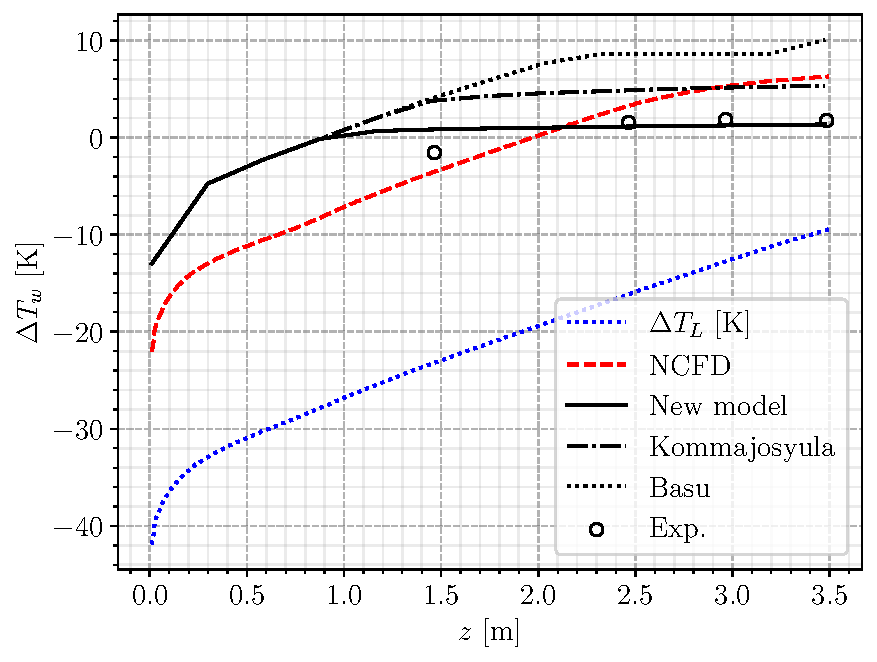
\includegraphics[width=0.6\linewidth]{img/HFP/test_allHFP_8Te44.pdf}
\caption{Comparison of different HFP on the 8G2P26W16Te49 DEBORA case.}
\label{fig:HFP_DEBORA}
\end{figure}

We see that the models perform in very different ways for the DEBORA conditions. Basu \etal formulation largely overestimates the experimental value while Kommajosyula's model finds a wall temperature slightly lower than the NCFD computation. On the other hand, the new formulation provides a wall temperature much closer to the experimental measurements, which is probably an effect mainly due to the large quenching combined with the pressure dependency of the nucleation site density.

\begin{remark*}{}
The wall-adjacent cell is located approximately at $y^{+} \approx 100$ which corresponds to a wall distance of roughly 0.3~mm. This could be considered a too short distance to extract the liquid temperature as input in the HFP model. 

\npar

However, the chosen case displays a large range of wall subcooling values (dotted blue line on Figure \ref{fig:HFP_DEBORA}) and the model appears to present very few variation while extracted value of $T_{L}$ increases by nearly $20\degC$. Sensitivity to the wall distance should nevertheless be further tested.
\end{remark*}



\section{Conclusions}

In this Chapter, we proposed different aspects of validation regarding the proposed Heat Flux Partitioning model developed in Section \ref{sec:hfp_new}. All in all, we can conclude that:

\begin{itemize}
\item The evolution of most physical parameters included in the model are coherent with detailed measurements conducted by Kossolapov \cite{kossolapov_experimental_2021} (Section \ref{sec:hfp_valid_fullkoss}), namely the nucleation site density, the bubble departure frequency, waiting time and quenching time.

\item The quenching seems overestimated with a probably too large sliding length. Meaning that the proposed modeling (\ie average distance between two nucleating bubbles, Section \ref{sec:sliding_length}) is likely to be an upper bound of the actual sliding length. Bubbles may actually slide over shorter length, which would require dedicated investigations when reaching boiling regimes with large bubble density on the wall.

\item The formulation seems able to capture different nature of heat flux partition, with high-quenching regimes at high pressure and low superheats (Figure \ref{fig:HFP_jens_BC}), regimes with both static and sliding coalescence at high pressure and high superheat (Figure \ref{fig:HFP_koss_BC}), or mixed between quenching and sliding coalescence at low to moderate pressure and high superheat (Figure \ref{fig:HFP_koss_BC}).

\item Wall temperature predictions (Section \ref{sec:hfp_valid_DTw}) using the new formulation along with reasonable values for the closing parameters $\parth{\theta,\ \dtheta,\ K }$ yields better results in average compared to older models. In particular, it seems capable of enhancing the wall temperature predictions on the DEBORA case as shown on Figure \ref{fig:HFP_DEBORA}.

\end{itemize}
